%-------------------------------------------------------------------------
% Design Project Input/Output Module Description
%-------------------------------------------------------------------------

\clearpage
\section{Force Input Module}
\label{sec-input-force}

This input module enables your IoT device to sense the amount of force
exerted on the surface of a squeeze pad. This may be useful in medical
devices, physical therapy, stress relief technology, virtual motion,
computer peripherals, touch-sensitive devices, etc. The sensor is a
variable resistor whose resistance depends on how much force is exerted
on the squeeze pad (e.g., squeezing it between two fingers); the
resistance is high (infinite) when there is no force and low when the
force is high.  The Arduino cannot directly sense resistance, but it can
sense an analog input voltage. We will use a simple circuit called a
voltage divider so that the voltage across the force sensor is
proportional to the resistance.

A sample circuit and Arduino code is shown below to get you started.
The circuit places a \wu{10}{k$\Omega$} resistor in series with the
force sensor so that voltage is divided between the two components. A
\wu{10}{k$\Omega$} resistor has brown-black-orange bands. We use a wire
to connect the node in between the resistor and the force sensor to an
analog input of the Arduino so that the Arduino can read the voltage
from one end of the \wu{10}{k$\Omega$} resistor to ground. The example
code will print the analog reading from the force sensor on the serial
monitor, similar to how we printed the analog reading from the grayscale
sensor in Lab~2. After setting up the circuit and programming the
Arduino, open the serial monitor and check how much force the sensor is
detecting. Then try squeezing the squeeze pad between two fingers. Does
the reading increase? Can you explain this behavior?

\vspace{0.1in}
\begin{minipage}[t]{0.49\tw}
  \vspace{0pt}

  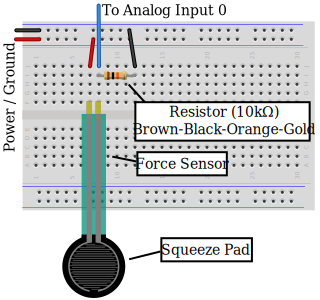
\includegraphics[width=\tw]{input-force-annotated.svg.pdf}
\end{minipage}
\hfill
\begin{minipage}[t]{0.49\tw}
  \vspace{0.1in}
  \begin{Verbatim}[gobble=3,fontsize=\small]
    int pin_force = A0;

    void setup() {
      Serial.begin(9600);
      pinMode( pin_force, INPUT );
    }

    void loop() {
      int force = analogRead( pin_force );

      Serial.println( force );
      delay(1000);
    }
  \end{Verbatim}
\end{minipage}
\vspace{0.1in}

%Questions:
